\documentclass[12pt]{article}
\usepackage{url,amsmath,amsthm,enumitem,amsfonts,tikz,verbatim,amssymb, wasysym,multicol,courier,sidecap,subcaption}
\usepackage[makeroom]{cancel}
\usetikzlibrary{arrows}

\title{Computing IV Project Portfolio}
\date{Fall 2018}
\author{Joel Savitz}

\usepackage{listings} %For code in appendix
\lstset
{ %Formatting for code in appendix
    language=c++,
    basicstyle=\footnotesize\ttfamily,
    numbers=left,
    stepnumber=1,
    showstringspaces=false,
    tabsize=1,
    breaklines=true,
    breakatwhitespace=false,
}

\begin{document}

\maketitle
\thispagestyle{empty}

\newpage

\tableofcontents

\listoffigures

\newpage

\section{Introduction}

\begin{figure}

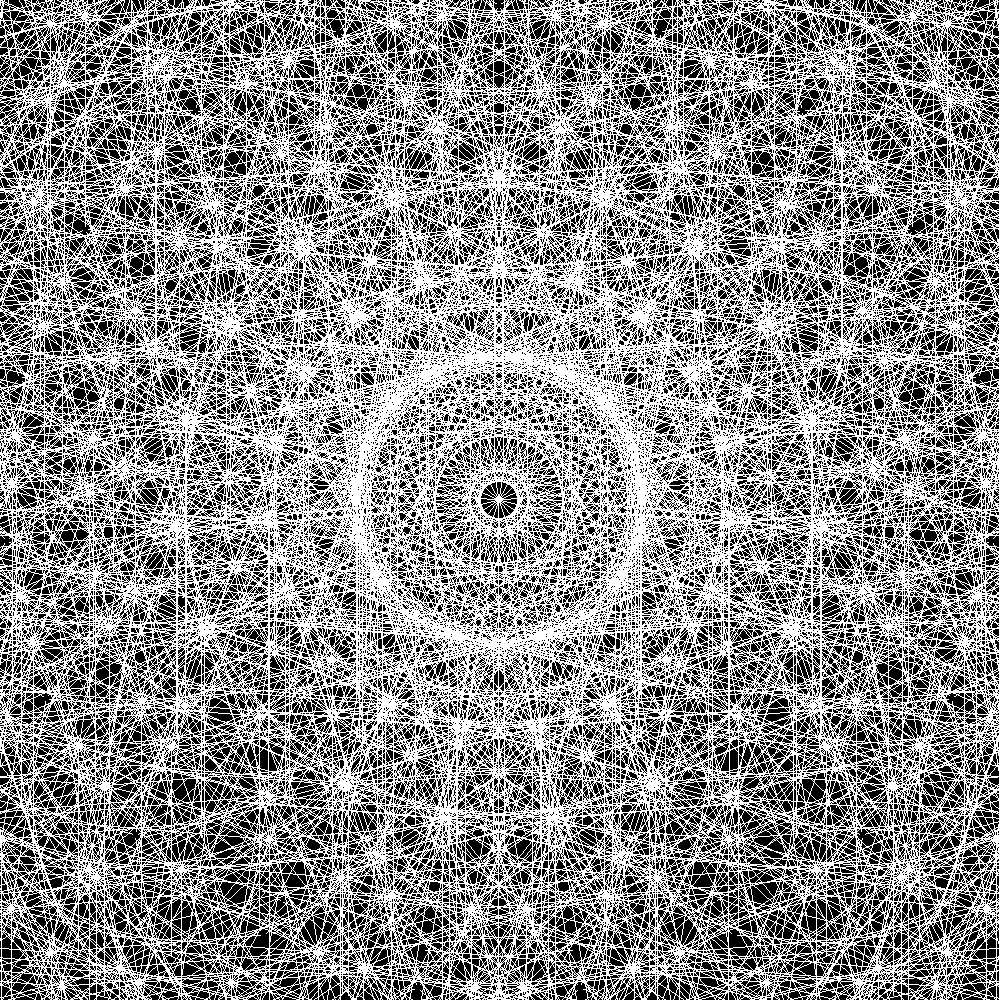
\includegraphics[scale=0.3]{../ps1_old/fractal_generator_example.png}
\centering

\caption{Output from a fractal generator I wrote in preparation for this class}

\end{figure}

I thoroughly enjoyed these projects. 

I will provide a short discussion of each project followed by it's source code.

Thank you Dr. Wilkes for approving and guiding me through an independent study of Computing IV. I gained a lot out of the practice with C++ that I believe will serve me well in my programming career.

\newpage

\section{PS0: Hello World with SFML}

The general idea of this assignment was as an introduction to the capabilities of SFML. First, I used supplied code to create a simple window with a circle in it. Then I modified the code to display a soccer ball, and added the ability for the user to modify the velocity of the ball using the arrow keys on the keyboard.

By setting the refresh rate of the window, I was able to create a loop that would change the position of the soccer ball by a variable velocity value in both the horizontal and vertical directions. I check if the new position of the ball would be outside of the border of the window, and if so, I reverse the velocity in that direction to simulate a bouncing effect. I also print the current velocity values at every refresh to standard output.

\begin{figure}

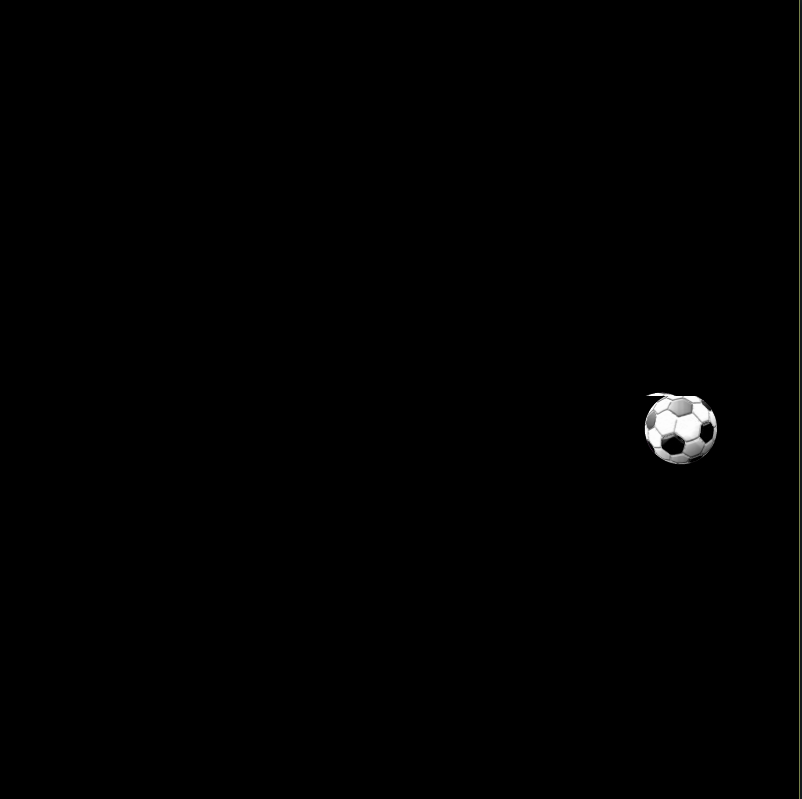
\includegraphics[scale=0.3]{../ps0/screenshot_tearing_due_to_simulated_motion}
\centering
\caption{My soccer ball sprite about to bounce off the side of the window}
\end{figure}

\subsection{\texttt{Makefile}}

\lstinputlisting[language=c++]{../ps0/Makefile}

\subsection{\texttt{main.cpp}}

\lstinputlisting[language=c++]{../ps0/main.cpp}

\newpage

\section{PS1: Recursive Graphics (Pythagoras Tree)}


\begin{figure}

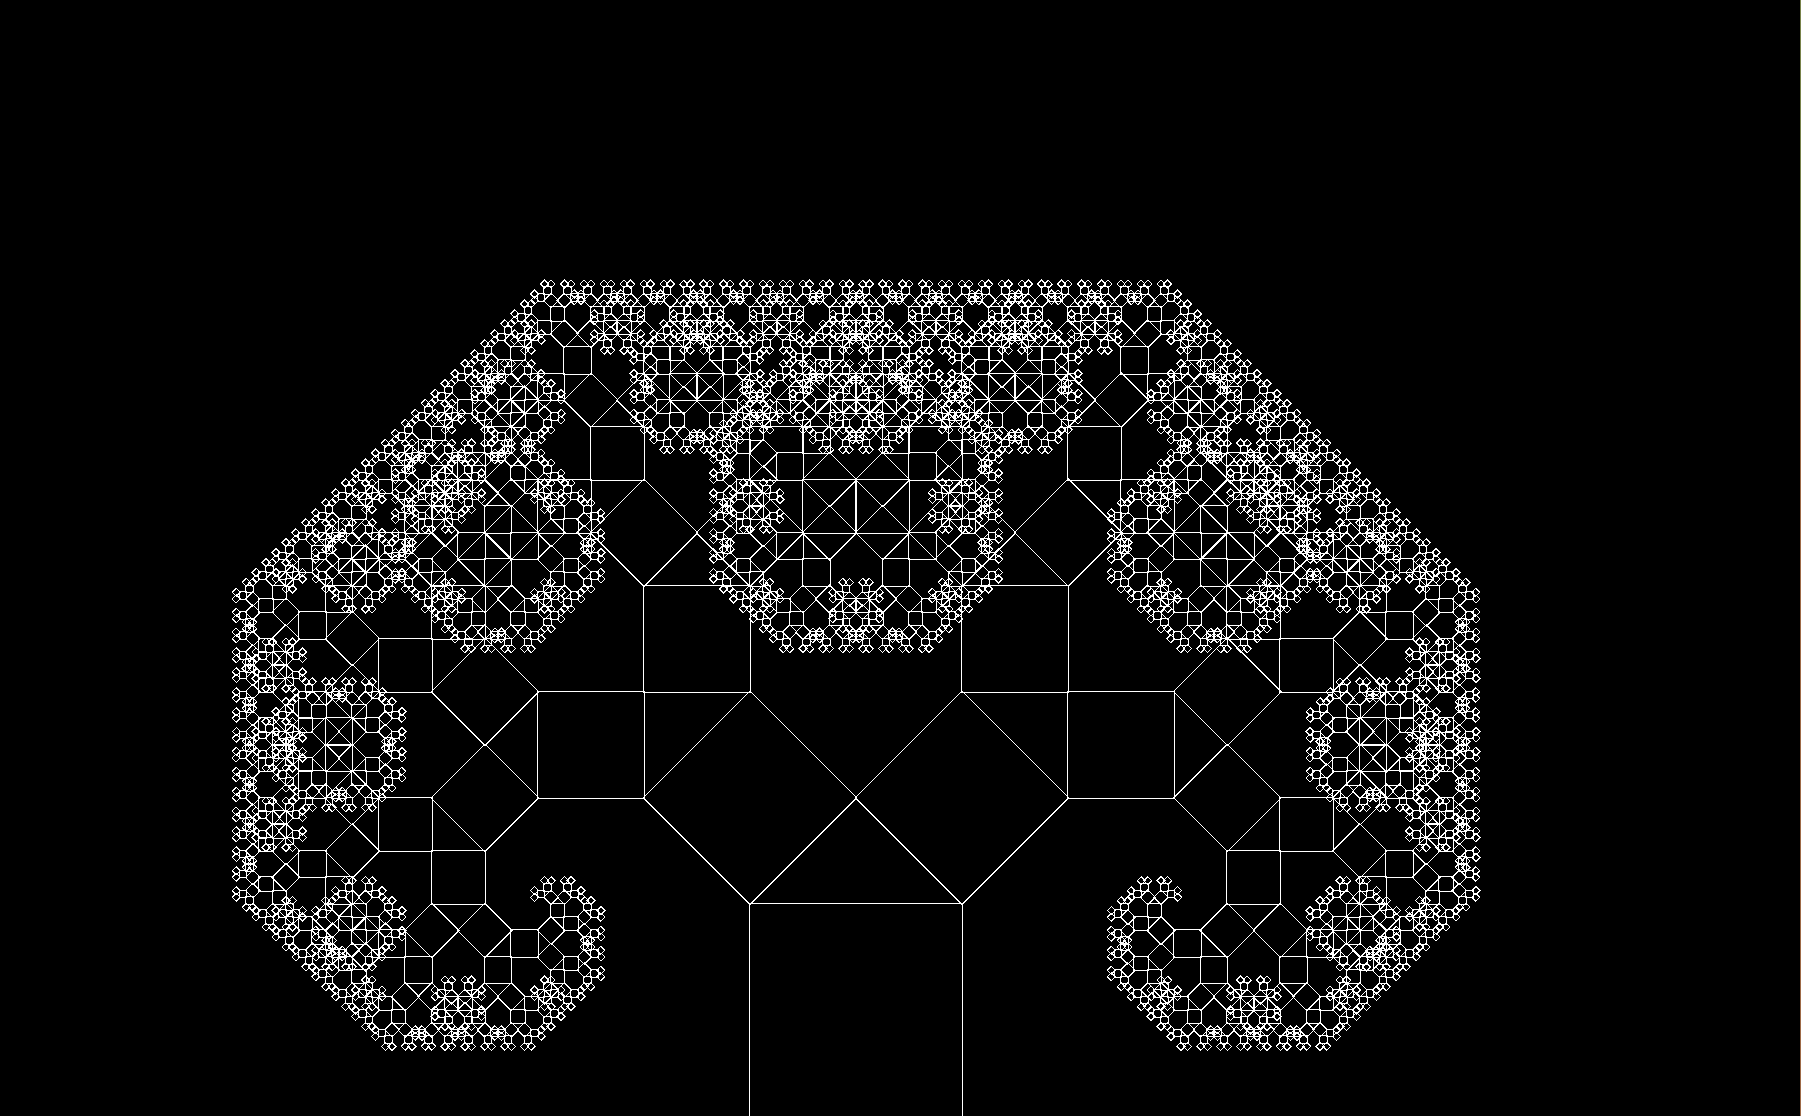
\includegraphics[scale=0.2]{../ps1/screenshot.png}
\centering
\caption{My Pythagoras tree}
\label{fig:pythagoras}
\end{figure}


For my recursive graphics assignment, I created a program that draws a Pythagoras tree, as can be seen in figure \ref{fig:pythagoras}. I modified this program to animate a folding-like rotation of the fractal, a stage of which can be seen in figure  \ref{fig:folded_pythagoras}.

Using basic trigonometry, I was able to implement this algorithm using recursive calls to functions that would draw squares relative to previously drawn squares. By modifying a key angle parameter at a certain rate relative to the screen refresh rate, I was able to simulate movement of the fractal.

The following keys can be used to interact with the program:

\begin{itemize}

\item[[ a]] Initiates a clockwise rotation/folding of the fractal.

\item [[ b]] Initiates a swaying animation of the fractal, like a tree in the wind.

\item [[ Left Arrow]] Increment the rotation of the fractal counterclockwise.

\item [[ Right Arrow]] Increment the rotation of the fractal clockwise.

\item[[ Spacebar]] Terminates any running animation.

\end{itemize}

\begin{figure}

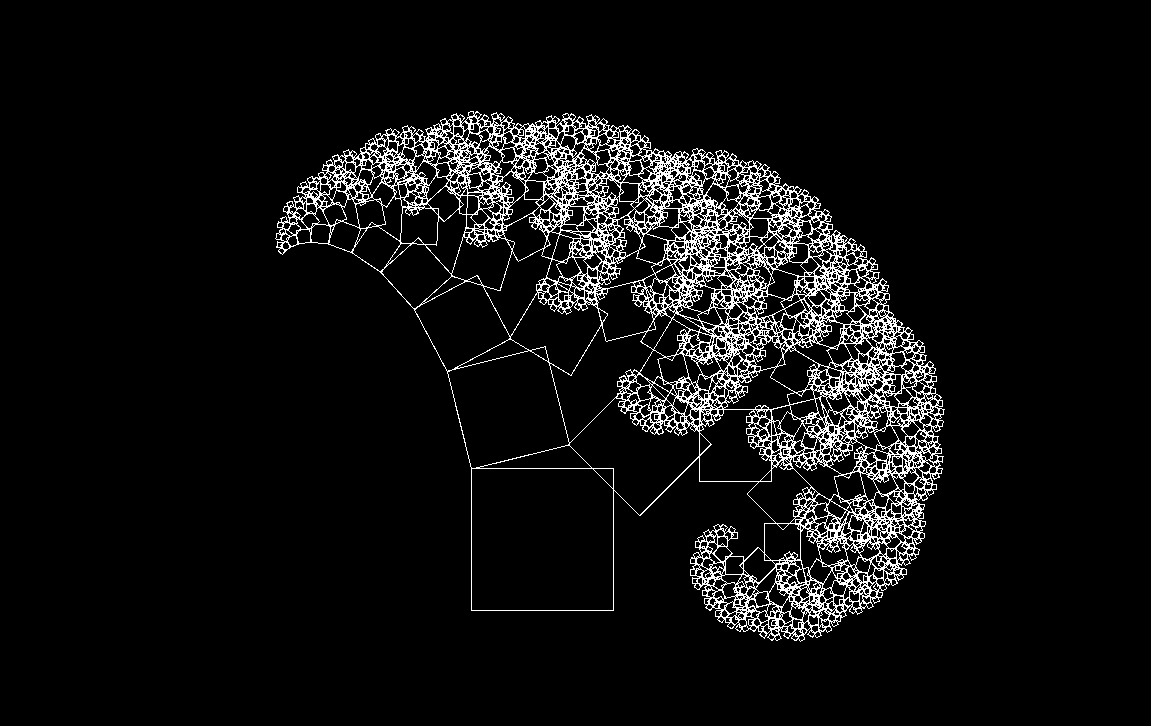
\includegraphics[scale=0.3]{../ps1/screenshot_folded.png}
\centering
\caption{My folded Pythagoras tree}
\label{fig:folded_pythagoras}
\end{figure}

\subsection{\texttt{Makefile}}

\lstinputlisting[language=c++]{../ps1/Makefile}

\subsection{\texttt{main.cpp}}

\lstinputlisting[language=c++]{../ps1/main.cpp}

\subsection{\texttt{PTree.hpp}}

\lstinputlisting[language=c++]{../ps1/PTree.hpp}

\subsection{\texttt{PTree.cpp}}

\lstinputlisting[language=c++]{../ps1/PTree.cpp}

\newpage

\section{PS2: Linear Feedback Shift Register and Image Encoding}

\begin{figure}
\centering
\begin{subfigure}{.5\textwidth}
  \centering
  \includegraphics[width=1\linewidth]{../ps2b/moon-encoded.png}
  \caption{Encoded moon graphic}
  \label{fig:moon-encoded}
\end{subfigure}%
\begin{subfigure}{.5\textwidth}
  \centering
  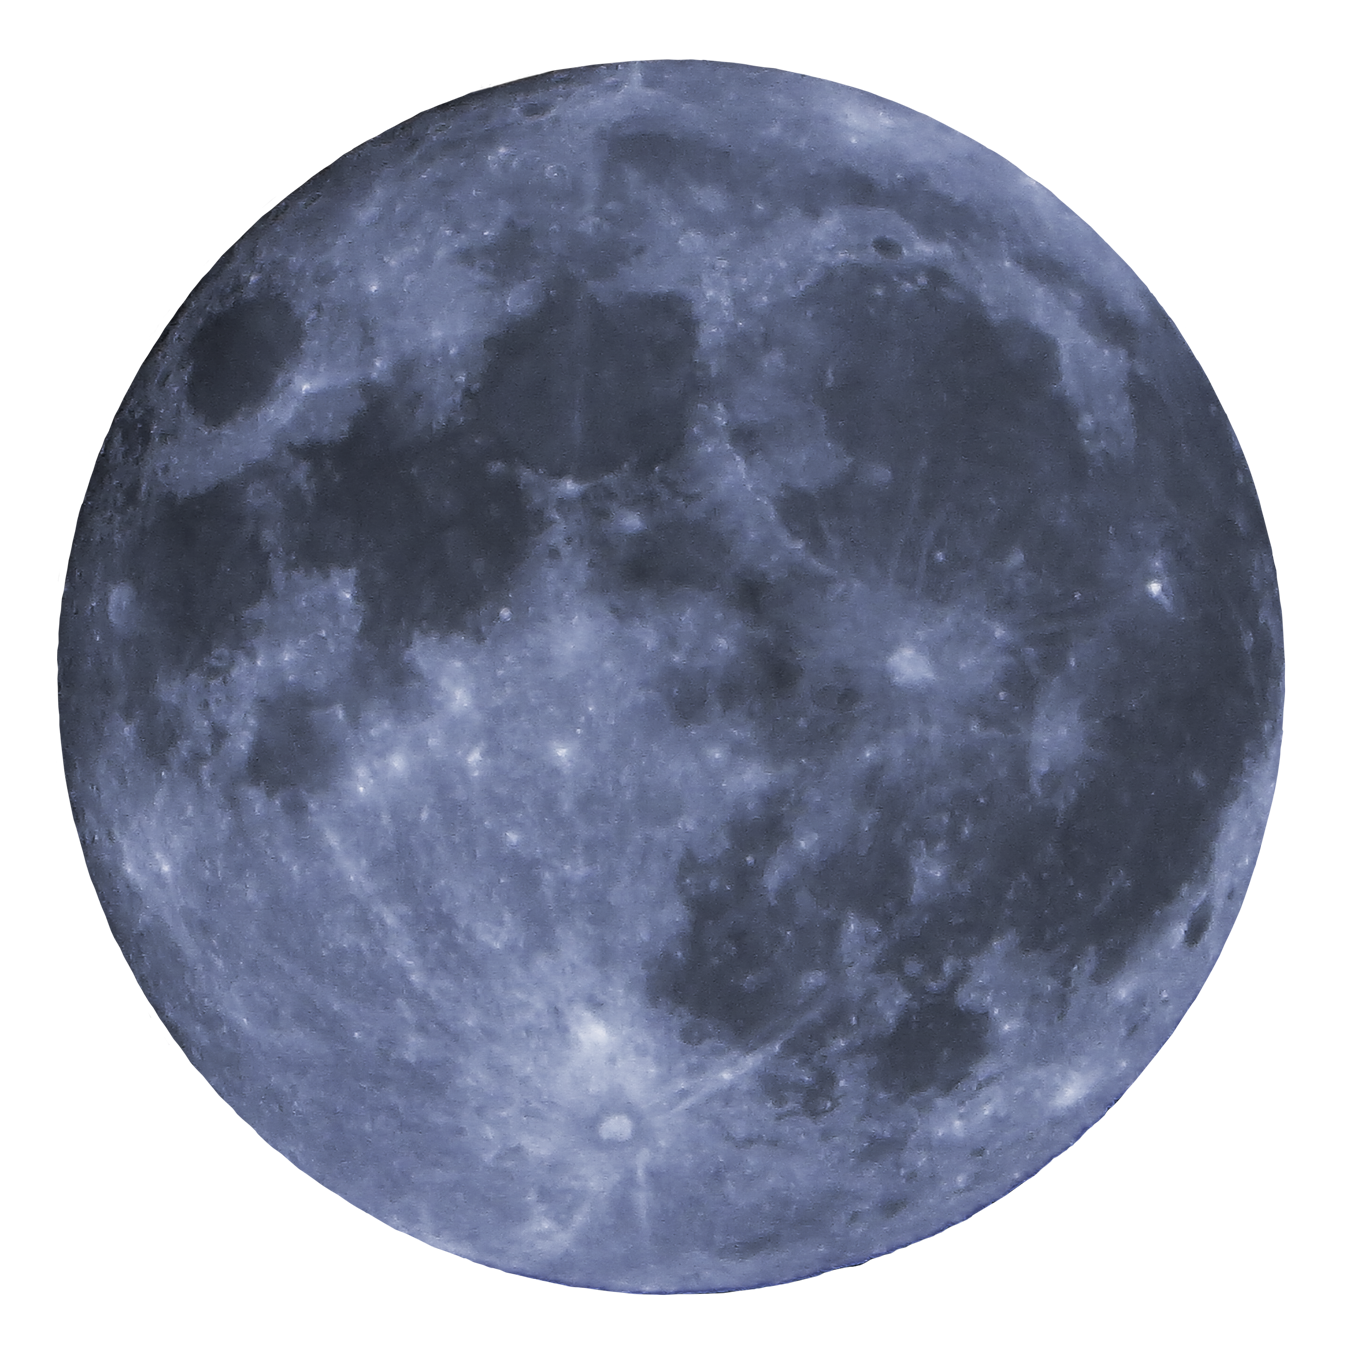
\includegraphics[width=1\linewidth]{../ps2b/moon-decoded.png}
  \caption{Decoded moon graphic}
  \label{fig:moon-decoded}
\end{subfigure}
\caption{PhotoMagic in action}
\label{fig:test}
\end{figure}

This assignment had two stages. First, I implemented a Linear Feedback Shift Register (``LFSR'') and tested it using the Boost unit test framework. Then, I used my LFSR to generate pseudo random values to encode a \texttt{png} file.

The LFSR requires an initial seed and tap value to run, and it is reversible, so running an image through the program with one set of parameters will output an image file that when passed as input to the program with the same parameters will output the original image. Figure \ref{fig:moon-encoded} demonstrates the output of running figure \ref{fig:moon-decoded} through the \texttt{PhotoMagic} executable. Figure \ref{fig:moon-decoded} is also the output of figure \ref{fig:moon-encoded} run through the program with the same parameters.

The seed is a binary bit string, and the tap value is a position in the string to use in the calculation of the pseudo-random values.

I learned about basic image encryption and gained some insight into how the \texttt{png} file format works. I also explore the Boost unit test framework, and the tests I wrote for my LFSR can be seen in section \ref{section:LFSR_test}.

\subsection{\texttt{Makefile}}

\lstinputlisting[language=c++]{../ps2b/Makefile}

\subsection{\texttt{PhotoMagic.cpp}}

\lstinputlisting[language=c++]{../ps2b/PhotoMagic.cpp}

\subsection{\texttt{LFSR.hpp}}

\lstinputlisting[language=c++]{../ps2b/LFSR.hpp}

\subsection{\texttt{LFSR.cpp}}

\lstinputlisting[language=c++]{../ps2b/LFSR.cpp}

\subsection{\texttt{test.cpp}}
\label{section:LFSR_test}

\lstinputlisting[language=c++]{../ps2a/test.cpp}

\newpage

\section{PS3: N-Body Simulation}

\begin{figure}

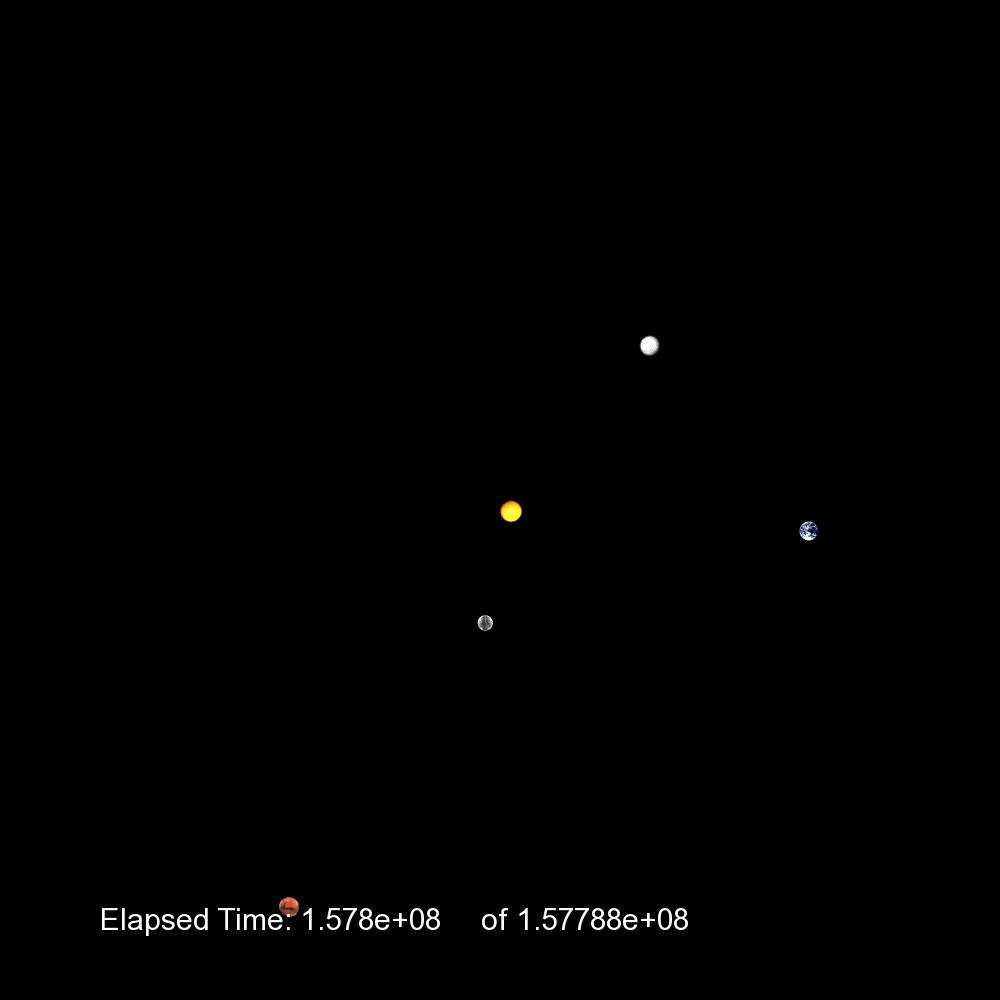
\includegraphics[scale=0.3]{../ps3b/screenshot.png}
\centering
\caption{The solar system in motion}
\label{fig:solar_system}
\end{figure}

For this assignment, I created a physics simulation of the gravitational particles acting on an arbitrary number of particles. The program takes an input file containing the initial state of the simulation and the names of sprite files to display for each particle. The total duration of the simulation as well as the time interval to simulate movement for each iteration of the loop is supplied via command line arguments.

When it is run, the program displays a window containing the particles and a display of the elapsed time out of the total time of the simulation, as seen in figure \ref{fig:solar_system}. Then, the simulation progresses until the total time has been reached, at which point the simulation freezes in that position and the program outputs the final state of the simulation to standard out.

I learned how to create basic physics simulations and gained some experience in program organization and debugging mathematical programs.

\subsection{\texttt{Makefile}}

\lstinputlisting[language=c++]{../ps3b/Makefile}

\subsection{\texttt{main.cpp}}

\lstinputlisting[language=c++]{../ps3b/main.cpp}

\subsection{\texttt{body.hpp}}

\lstinputlisting[language=c++]{../ps3b/body.hpp}

\subsection{\texttt{body.cpp}}

\lstinputlisting[language=c++]{../ps3b/body.cpp}

\newpage

\section{PS5: Ring Buffer and Guitar Hero}

\begin{figure}

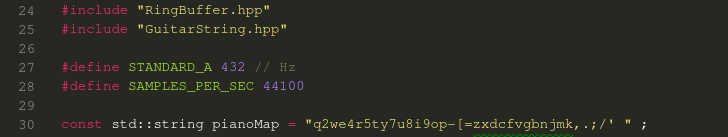
\includegraphics[scale=0.6]{../ps5b/keymapping.png}
\centering
\caption{The definition of my keyboard used to play guitar sounds}
\label{fig:piano_map}
\end{figure}

\begin{figure}
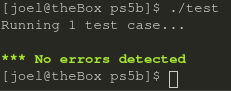
\includegraphics[scale=0.6]{../ps5b/passes.png}
\centering
\caption{My PS5b code passing the tests defined in GStest.cpp}
\end{figure}

For my final assignment, I created a basic guitar synthesizer using the Karplus-Strong algorithm to simulate vibrations of a guitar string given a random seed. Using the keymappings defined in the code visible in figure \ref{fig:piano_map}, the user can input different frequencies that will be played, ranging from 110 Hz to 880 Hz, and the program will will create the sound by passing a frequency parameter to the GuitarString object, which returns samples that can be used as a sound buffer to play a noise that sounds like a guitar playing the note that corresponds to that frequency.

The assignment taught be the basics of electronic musical synthesis and about the audio capabilities of SFML, an aspect which I had not yet explored. I also wrote unit tests for my GuitarString class which can be seen in section \ref{section:guitar_test}.

\subsection{\texttt{Makefile}}

\lstinputlisting[language=c++]{../ps5b/Makefile}

\subsection{\texttt{GuitarHero.cpp}}

\lstinputlisting[language=c++]{../ps5b/GuitarHero.cpp}

\subsection{\texttt{GuitarString.hpp}}

\lstinputlisting[language=c++]{../ps5b/GuitarString.hpp}

\subsection{\texttt{GuitarString.cpp}}

\lstinputlisting[language=c++]{../ps5b/GuitarString.cpp}

\subsection{\texttt{RingBuffer.hpp}}

\lstinputlisting[language=c++]{../ps5b/RingBuffer.hpp}

\subsection{\texttt{RingBuffer.cpp}}

\lstinputlisting[language=c++]{../ps5b/RingBuffer.cpp}

\subsection{\texttt{test.cpp}}
\label{section:guitar_test}

\lstinputlisting[language=c++]{../ps5a/test.cpp}


\newpage
\section{Airport Concurrency Simulation}

\begin{figure}

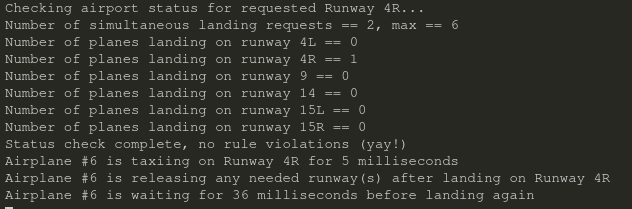
\includegraphics[scale=0.6]{../airport/Airport-Sync/simulation.png}
\centering
\caption{Airport simulation in progress}
\end{figure}

This assignment was very different than the rest. I was given a functioning program that did not handle concurrent threads properly and I had to tweak it to properly handle concurrency. The program simulates a number of airplanes landing at Logan Airport on different runways, where some runways cannot be used at the same time as others because they physically overlap. This structure is used to represent different threads requiring exclusive use of different resources at different times.

Given rules stating which runways must be free before a runway can be used, I forced every plane landing on a runway to get a mutex lock on all prerequisite runways, and I enforced a total ordering on the calls to mutex lock and unlock in order to avoid a deadlock. I also used a condition variable to prevent more than six airplane threads from requesting a landing at the same time.

In order to complete this assignment, I had to familiarize myself with the C++ threading library and with basic concurrency problems. I gained experience debugging basic multi-threaded programs.

\subsection{\texttt{Makefile}}

\lstinputlisting[language=c++]{../airport/Airport-Sync/Makefile}

\subsection{\texttt{Airport.cpp}}

\lstinputlisting[language=c++]{../airport/Airport-Sync/Airport.cpp}

\subsection{\texttt{AirportServer.hpp}}

\lstinputlisting[language=c++]{../airport/Airport-Sync/AirportServer.h}

\subsection{\texttt{AirportServer.cpp}}

\lstinputlisting[language=c++]{../airport/Airport-Sync/AirportServer.cpp}

\end{document}
